\documentclass{article}

\usepackage{cancel}
\usepackage{amsmath}
\usepackage[includehead,nomarginpar]{geometry}
\usepackage{graphicx}
\usepackage{amsfonts} 
\usepackage{verbatim}
\usepackage{mathrsfs}  
\usepackage{lmodern}
\usepackage{braket}
\usepackage{bookmark}
\usepackage{fancyhdr}
\usepackage{romanbarpagenumber}
\usepackage{minted}
%\usepackage{subfig}
\usepackage[italian]{babel}
\usepackage{float}
%\usepackage{wrapfig}
%\usepackage[export]{adjustbox}
\usepackage{graphicx}
\allowdisplaybreaks

\setlength{\headheight}{12.0pt}
\addtolength{\topmargin}{-12.0pt}
\graphicspath{ {../Immagini/} }

\hypersetup{
    colorlinks=true,
    linkcolor=black,
}

\newsavebox{\tempbox} %{\raisebox{\dimexpr.5\ht\tempbox-.5\height\relax}}

\makeatother

\numberwithin{equation}{section}
\newcommand{\tageq}{\tag{\stepcounter{equation}\theequation}}
\newcommand{\vv}[1]{\verb{\text{#1}}}
\AtBeginDocument{%
  \renewcommand{\figurename}{Fig.}
}
\fancypagestyle{link}{\fancyhf{}\renewcommand{\headrulewidth}{0pt}\fancyfoot[C]{Sorgente del file LaTeX disponibile al seguente link: \url{https://github.com/00Darxk/Intelligenza-Artificiale-e-Machine-Learning}}}

\begin{document}

\title{%
    \textbf{Intelligenza Artificiale e Machine Learning}  \\ 
    \large Esercizi Svolti di Intelligenza Artificiale e Machine Learning \\
    \textit{Anno Accademico: 2024/25}}
\author{\textit{Giacomo Sturm}}
\date{\textit{Dipartimento di Ingegneria Civile, Informatica e delle Tecnologie Aeronautiche \\
Università degli Studi ``Roma Tre"}}

\maketitle
\thispagestyle{link}

\clearpage


\pagestyle{fancy}
\fancyhead{}\fancyfoot{}
\fancyhead[C]{\textit{Intelligenza Artificiale e Machine Learning - Università degli Studi ``Roma Tre"}}
\fancyfoot[C]{\thepage}
\pagenumbering{Roman}

\tableofcontents

\clearpage
\pagenumbering{arabic}

\section{Esercitazione 13/11/24}

\subsection*{Esercizio 1}

Dato il seguente Spazio degli Stati: $s_0,s_1,s_2,s_3,s_4,s_5$, con stato iniziale $s_0$, e stato obiettivo $s_5$. 
Questi stati sono collegati da certi operatori di costo:
\begin{itemize}
    \item $F$: costo 3. $F(s_0)=s_2, F(s_1)=s_3, F(s_4)=s_5$;
    \item $G$: costo 4. $G(s_3)=s_2, G(s_3)=s_4, G(s_4)=s_3$;
    \item $H$: costo 5; $H(s_0)=s_1, H(s_2)=s_0, H(s_2)=s_4, H(s_4)=s_2, H(s_5)=s_1$;
    \item $I$: costo 6; $I(s_3)=s_5$.
\end{itemize}
Nel modo seguente: 

\begin{figure}[H]%
    \centering%
    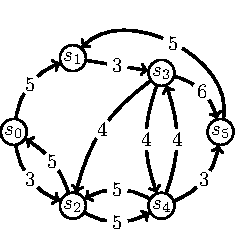
\includegraphics[scale=1.2]{grafo_esercitazione_1.pdf}%
\end{figure}
E la seguente funzione euristica: $h(s_0)=10$, $h(s_1)=6$, $h(s_2)=7$, $h(s_3)=4$, $h(s_4)=5$, $h(s_5)=0$. 

\begin{enumerate}
    \item Eseguire l'algoritmo A* con modalità tree-search, fino alla terminazione disegnando l'albero di ricerca, riportando per ogni passo il 
contenuto della frontiera, il nodo scelto per l'espansione ed i nodi generati;
    \item Riportare la soluzione trovata dell'algoritmo, indicando se tale soluzione è o non è quella ottima e indicando se la funzione euristica 
$h$ rispetta la condizione di ammissibilità (motivare la risposta). 
\end{enumerate}

\subsubsection*{Domanda 1}

Bisogna specificare i vari passi ottenuti dall'algoritmo A*, specificando la frontiera i nodi contenuti ed espansi ed il nodo successivo 
da espandere.

\begin{enumerate}
    \item Nella frontiera è presente solamente lo stato iniziale $[s_0]$;
    \item Si espande lo stato iniziale $s_0$, nella frontiera si ha $[s_2,s_1]$, dove $f(s_2)=3+7$ e $f(s_1)=5+6$;
    \item Si espande il nodo $s_2$, con $f(s_2)=10$, per cui nella frontiera entra il nodo $s_4$: $[s_1,s_4]$, con $f(s_1)=5+6$ e $f(s_4)=8+5$;
    \item Si espande il nodo $s_1$, con $f(s_1)=12$, per cui nella frontiera entra il nodo $s_3$: $[s_3, s_4]$, con $f(s_3)=8+4$ e $f(s_4)=8+5$;
    \item Si espande il nodo $s_3$, con $f(s_3)=12$, per cui nella frontiera entra il nodo $s_5$: $[s_4, s_5]$, con $f(s_4)=8+5$ e $f(s_5)=14+0$;
    \item Si espande il nodo $s_4$, con $f(s_4)=13$, per cui nella frontiera entra il nodo $s_5$: $[s_5]$, con $f(s_5)=11+0$;
    \item Si espande il nodo $s_5$, con $f(s_5)=11$. Questo nodo è il nodo obiettivo, quindi l'algoritmo termina. 
\end{enumerate}

%% TODO fix frontiera con tutti i nodi in frontiera

I nodi rossi sono quelli nella frontiera, i nodi blu sono i nodi nella frontiera da espandere:

\begin{figure}[H]%
    \centering%
    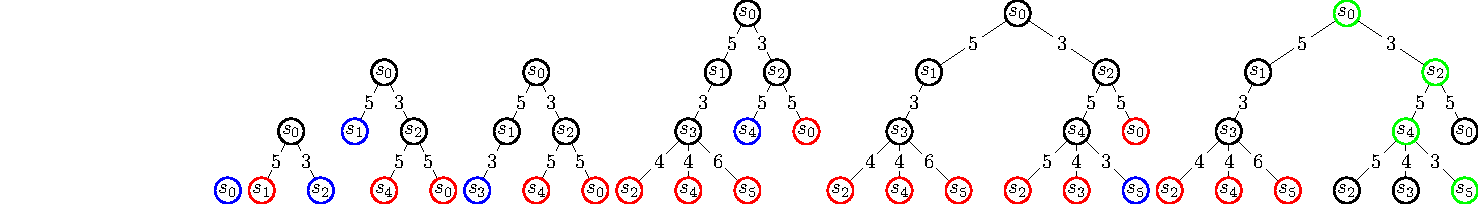
\includegraphics[trim={3.9cm 0 0 0}, scale=0.95]{albero_esercitazione_1.pdf}%
\end{figure}

\subsubsection*{Domanda 2}

La soluzione dell'algoritmo è $s_0,s_2,s_4,s_5$, di costo 11:
\begin{figure}[H]%
    \centering%
    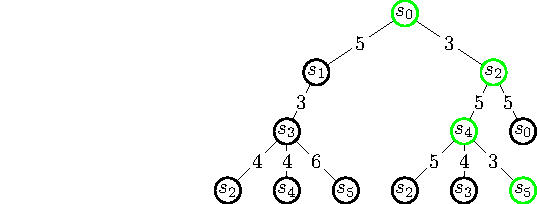
\includegraphics[trim={4cm 0 0 0}]{soluzione_esercitazione_1.pdf}%
\end{figure}

La funzione euristica $h$ utilizzata è maggiore del costo effettivo per il nodo $s_4$: 
\begin{equation}
    h(s_4)=5>3=h^*(s_4,s_5)
\end{equation}

Quindi non è una funzione ammissibile. La soluzione trovata 
non è garantito sia la soluzione ottima. 

\subsection*{Esercizio 2}

Scrivere il codice Python per la gestione di una lista concatenata ordinata, avvalendosi delle classi. \\
\begin{minted}{python}
    class Node:
        def __init__(self, data, next)
            self.__data = data
            self.__next = next

    class List:
        def __init__(self):
            self.__head = None
            self.__tail = None

        def add(self, newNode):            
            if self.__head == None or self.__head.data > newNode.data:
                if self.__head == None:
                    self.__tail = newNode
                newNode.next = self.__head
                self.__head = newNode

            elif self.__tail.data < newNode.data:
                if self.__tail != None:
                    self.__tail.next = newNode
                if self.__head == None:
                    self.__head = NewNode
                self.__tail = newNode

            else:            
                p = self.__head
                while p.next != None and p.data < newNode.data:
                    p = p.next
                newNode.next = p.next
                p.next = newNode
\end{minted}

\subsection*{Esercizio 3}

Illustrare nel dettaglio l'algoritmo ``Greedy'', presentando il codice Python, opportunamente commentato per il problema della ricerca di un 
itinerario. \\
\begin{minted}{python}
    def Greedy_Best_First():
        fringe = SortedLinkedList() 

        initialState = State()
        
        root = Node(initialState, None, h[initialState.name])
        fringe.add(Item(root.h, root))
    
        while not fringe.is_empty():
            itemRemoved = fringe.remove_front()
            currentNode = itemRemoved.node

            if currentNode.state.checkGoalState():
                currentNode.state.printPath()
                break
            else: 
                childStates = currentNode.state.successorFunction()
                for childState in childStates:
                    childNode = Node(State(childState), currentNode, 
                                        h[State(childState).name])
                    fringe.add(Item(childNode.h, childNode))
\end{minted}

\end{document}